%\makeindex
\chapter{Vegetation}




%%%%%%%%%%%%%%%%%%%%%%%%%%%%%%%%%%%%%%%%%%%%%%%%%%%%%%%%%%%%%%%
\section{Input}
%%%%%%%%%%%%%%%%%%%%%%%%%%%%%%%%%%%%%%%%%%%%%%%%%%%%%%%%%%%%%%%

\subsection{Parameters}
\begin{center}
\begin{longtable}{|p {3.4 cm}|p {4.7 cm}|p {1. cm}|p{0.8 cm}|p{1.4 cm}|p{0.8 cm}|p{1.3 cm}|}
\hline
\textbf{Keyword} & \textbf{Description} & \textbf{M. U.} & \textbf{range} & \textbf{Default Value} & \textbf{Sca / Vec} & \textbf{Str / Num / Opt} \\ \hline
\endfirsthead
\hline
\multicolumn{7}{| c |}{continued from previous page} \\
\hline
\textbf{Keyword} & \textbf{Description} & \textbf{M. U.} & \textbf{range} & \textbf{Default Value} & \textbf{Sca / Vec} & \textbf{Str / Num / Opt} \\ \hline
\endhead
\hline
\multicolumn{7}{| c |}{{continued on next page}}\\ 
\hline
\endfoot
\endlastfoot
\hline
VegHeight \index{VegHeight} & vegetation height & mm & 50, 2000 & 1000 & vec & num \\ \hline
LSAI \index{LSAI} & Leaf and Stem Area Index [$L^2/L^2$] & - & 0, 1 & 1 & vec & num\\ \hline
CanopyFraction \index{CanopyFraction} & Canopy fraction [0: no canopy in the pixel, 1: pixel fully covered by canopy] & - & 0, 1 & 0 & vec & num \\ \hline
DecayCoeffCanopy \index{DecayCoeffCanopy} & Decay coefficient of the eddy diffusivity profile in the canopy & - & 0, inf & 2.5 & vec & num \\ \hline
VegSnowBurying \index{VegSnowBurying} & Coefficient of the exponential snow burying of vegetation & - & 0, inf & 1 & vec & num \\ \hline
RootDepth \index{RootDepth} & Root depth (it is used to calculate root\_fraction for each layer, it must be positive) & mm & 0, inf & 300 & vec & num \\ \hline
MinStomatalRes \index{MinStomatalRes} & Minimum stomatal resistance & s $m^{-1}$ & 0, inf & 60 & vec & num \\ \hline
VegReflectVis \index{VegReflectVis} & Vegetation reflectivity in the visible & - & 0, 1 & 0.2 & vec & num \\ \hline
VegReflNIR \index{VegReflNIR} & Vegetation reflectivity in the near infrared & - & 0, 1 & 0.2 & vec & num \\ \hline
VegTransVis \index{VegTransVis} & Vegetation transmissimity in the visible & - & 0, 1 & 0.2 & vec & num \\ \hline
VegTransNIR \index{VegTransNIR} & Vegetation transmissimity in the near infrared & - & 0, 1 & 0.2 & vec & num \\ \hline
LeafAngles \index{LeafAngles} & Departure of leaf angles from a random distribution (1 horizontal, 0 random, -1 vertical) & - & -1, 0, 1 & 0 & vec & opt \\ \hline
CanDensSurface \index{CanDensSurface} & Surface density of canopy & kg m$^{-2}$ LSAI$^{-1}$ & 0, inf & 2 & vec & num \\ \hline
\caption{{Keywords of vegetation characteristics that may be set in geotop.inpts. Each parameter may be given in input as a vector, each component representing the value corresponding to the LandCoverMapFile value identified by the vector index}}
\label{veg_LC_vector}
\end{longtable}
\end{center}

\section{Numerics}
\begin{center}
\begin{longtable}{|p {3.5 cm}|p {5 cm}|p {1 cm}|p{1 cm}|p{1.1 cm}|p{1.cm}|p{1 cm}|}
\hline
\textbf{Keyword} & \textbf{Description} & \textbf{M. U.} & \textbf{range} & \textbf{Default Value} & \textbf{Scalar / Vector} & \textbf{Logical / Numeric} \\ \hline
\endfirsthead
\hline
\multicolumn{7}{| c |}{continued from previous page} \\
\hline
\textbf{Keyword} & \textbf{Description} & \textbf{M. U.} & \textbf{range} & \textbf{Default Value} & \textbf{Sca / Vec} & \textbf{Log / Num} \\ \hline
\endhead
\hline
\multicolumn{7}{| c |}{{continued on next page}}\\ 
\hline
\endfoot
\endlastfoot
\hline
CanopyMaxIter \index{CanopyMaxIter} & Max number of iterations for (vegetation energy balance equation) &  &  & 3 & sca & num \\ \hline
LocMaxIter \index{LocMaxIter} & Max number of iterations for the calculation of the within-canopy Monin-Obukhov length (vegetation energy balance equation) & - &  & 3 & sca & num \\ \hline
TsMaxIter \index{TsMaxIter} & Max number of iterations for the calculation of canopy air temperature (vegetation energy balance equation) & - &  & 2 & sca & num \\ \hline
CanopyStabCorrection \index{CanopyStabCorrection} & Use of the stability corrections within canopy (=1), otherwise (=0) & - &  & 1 & sca & opt \\ \hline
BusingerMaxIter \index{BusingerMaxIter} & Max number of iterations for Monin-Obulhov stability algorithm -Businger parameterization (surface energy balance equation) & - &  & 5 & sca & num \\ \hline
\caption{Keywords of input numeric parameters for the energy equation regarding vegetation routines settable in geotop.inpts}
\label{numeric1d_num_veg}
\end{longtable}
\end{center}

%%%%%%%%%%%%%%%%%%%%%%%%%%%%%%%%%%%%%%%%%%%%%%%%%%%%%%%%%%%%%%%
\section{Output}
%%%%%%%%%%%%%%%%%%%%%%%%%%%%%%%%%%%%%%%%%%%%%%%%%%%%%%%%%%%%%%%

\subsection{Point}
\subsubsection{Files}

\begin{center}
\begin{longtable}{|p {5.0 cm}|p {9 cm}|}
\hline
\textbf{Keyword} & \textbf{Description}  \\ \hline
\endfirsthead
\hline
\multicolumn{2}{| c |}{continued from previous page} \\
\hline
\textbf{Keyword} & \textbf{Description}   \\ \hline
\endhead
\hline
\multicolumn{2}{| c |}{{continued on next page}}\\ 
\hline
\endfoot
\endlastfoot
\hline
TimeDependentVegetationParameterFile \index{TimeDependentVegetationParameterFile} & name of the file providing the time dependent vegetation parameters \\ \hline
PointOutputFile \index{PointOutputFile} & name of the file providing the properties for the simulation point \\ \hline
PointOutputFileWriteEnd \index{PointOutputFileWriteEnd} & name of the output file providing the Point values written just once at the end \\ \hline
\caption{Keywords of file related to vegetation}
\label{veget_file}
\end{longtable}
\end{center}



\subsubsection{Headers}

\begin{center}
\begin{longtable}{|p {4.4 cm}|p {6.5 cm}|p {2 cm}|}
\hline
\textbf{Keyword} & \textbf{Description} & \textbf{Associated file}  \\ \hline
\endfirsthead
\hline
\multicolumn{3}{| c |}{continued from previous page} \\
\hline
\textbf{Keyword} & \textbf{Description} & \textbf{Associated file}  \\ \hline
\endhead
\hline
\multicolumn{3}{| c |}{{continued on next page}}\\ 
\hline
\endfoot
\endlastfoot
\hline
HeaderTvegPoint \index{HeaderTvegPoint} & column name in the file PointOutputFile for the variable TvegPoint & PointOutputFile  \\ \hline
HeaderTCanopyAirPoint \index{HeaderTCanopyAirPoint} & column name in the file PointOutputFile for the variable TCanopyAirPoint & PointOutputFile  \\ \hline
HeaderLSAIPoint \index{HeaderLSAIPoint} & column name in the file PointOutputFile for the variable LSAIPoint & PointOutputFile  \\ \hline
Headerz0vegPoint \index{Headerz0vegPoint} & column name in the file PointOutputFile for the variable z0vegPoint & PointOutputFile \\ \hline
Headerd0vegPoint \index{Headerd0vegPoint} & column name in the file PointOutputFile for the variable d0vegPoint & PointOutputFile  \\ \hline
HeaderEstoredCanopyPoint \index{HeaderEstoredCanopyPoint} & column name in the file PointOutputFile for the variable EstoredCanopyPoint & PointOutputFile  \\ \hline
HeaderSWvPoint \index{HeaderSWvPoint} & column name in the file PointOutputFile for the variable SWvPoint & PointOutputFile  \\ \hline
HeaderLWvPoint \index{HeaderLWvPoint} & column name in the file PointOutputFile for the variable LWvPoint & PointOutputFile  \\ \hline
HeaderHvPoint \index{HeaderHvPoint} & column name in the file PointOutputFile for the variable HvPoint & PointOutputFile  \\ \hline
HeaderLEvPoint \index{HeaderLEvPoint} & column name in the file PointOutputFile for the variable LEvPoint & PointOutputFile  \\ \hline
HeaderHgUnvegPoint \index{HeaderHgUnvegPoint} & column name in the file PointOutputFile for the variable HgUnvegPoint & PointOutputFile  \\ \hline
HeaderLEgUnvegPoint \index{HeaderLEgUnvegPoint} & column name in the file PointOutputFile for the variable LEgUnvegPoint & PointOutputFile  \\ \hline
HeaderHgVegPoint \index{HeaderHgVegPoint} & column name in the file PointOutputFile for the variable HgVegPoint & PointOutputFile  \\ \hline
HeaderLEgVegPoint \index{HeaderLEgVegPoint} & column name in the file PointOutputFile for the variable LEgVegPoint & PointOutputFile  \\ \hline
HeaderEvapSurfacePoint \index{HeaderEvapSurfacePoint} & column name in the file PointOutputFile for the variable EvapSurfacePoint & PointOutputFile \\ \hline
HeaderTraspCanopyPoint \index{HeaderTraspCanopyPoint} & column name in the file PointOutputFile for the variable TraspCanopyPoint & PointOutputFile  \\ \hline
HeaderWaterOnCanopyPoint \index{HeaderWaterOnCanopyPoint} & column name in the file PointOutputFile for the variable WaterOnCanopyPoint & PointOutputFile  \\ \hline
HeaderSnowOnCanopyPoint \index{HeaderSnowOnCanopyPoint} & column name in the file PointOutputFile for the variable SnowOnCanopyPoint & PointOutputFile  \\ \hline
HeaderQVegPoint \index{HeaderQVegPoint} & column name in the file PointOutputFile for the variable specific humidity near the vegetation & PointOutputFile  \\ \hline
HeaderLObukhovCanopyPoint \index{HeaderLObukhovCanopyPoint} & column name in the file PointOutputFile for the variable LObukhovCanopyPoint & PointOutputFile \\ \hline
HeaderWindSpeedTopCanopyPoint \index{HeaderWindSpeedTopCanopyPoint} & column name in the file PointOutputFile for the variable WindSpeedTopCanopyPoint & PointOutputFile  \\ \hline
HeaderDecayKCanopyPoint \index{HeaderDecayKCanopyPoint} & column name in the file PointOutputFile for the variable DecayKCanopyPoint & PointOutputFile \\ \hline
\caption{Keywords of the personalized headers for the PointOutputFile}
\label{vegetation_pointoutput}
\end{longtable}
\end{center}

\subsubsection{Parameters}

\begin{center}
\begin{longtable}{|p {3.6 cm}|p {4.9 cm}|p {1 cm}|p{1. cm}|p{1.1 cm}|p{1. cm}|p{1 cm}|}
\hline
\textbf{Keyword} & \textbf{Description} & \textbf{M. U.} & \textbf{range} & \textbf{Default Value} & \textbf{Sca / Vec} & \textbf{Log / Num} \\ \hline
\endfirsthead
\hline
\multicolumn{7}{| c |}{continued from previous page} \\
\hline
\textbf{Keyword} & \textbf{Description} & \textbf{M. U.} & \textbf{range} & \textbf{Default Value} & \textbf{Sca / Vec} & \textbf{Log / Num} \\ \hline
\endhead
\hline
\multicolumn{7}{| c |}{{continued on next page}}\\ 
\hline
\endfoot
\endlastfoot
\hline
DefaultPoint \index{DefaultPoint} & 0: use personal setting, 1:use default & - & 0, 1 & 1 & sca & opt \\ \hline
DtPlotPoint \index{DtPlotPoint} & Plotting Time step (in hour) of the output for specified pixels (0 means the it is not plotted) & h & 0, inf & 0 & vec & num \\ \hline
DatePoint \index{DatePoint} & column number in which one would like to visualize the Date12[DDMMYYYY hhmm]    	 & - & 1, 76 & -1 & sca & num \\ \hline
JulianDayFromYear0Point \index{JulianDayFromYear0Point} & column number in which one would like to visualize the JulianDayFromYear0[days]   	 & - & 1, 76 & -1 & sca & num \\ \hline
TimeFromStartPoint \index{TimeFromStartPoint} & column number in which one would like to visualize the TimeFromStart[days]  & - & 1, 76 & -1 & sca & num \\ \hline
PeriodPoint \index{PeriodPoint} & column number in which one would like to visualize the Simulation\_Period & - & 1, 76 & -1 & sca & num \\ \hline
RunPoint \index{RunPoint} & column number in which one would like to visualize the Run	 & - & 1, 76 & -1 & sca & num \\ \hline
IDPointPoint \index{IDPointPoint} & column number in which one would like to visualize the IDpoint  & - & 1, 76 & -1 & sca & num \\ \hline
TvegPoint \index{TvegPoint} & column number in which one would like to visualize the Tvegetation[\textcelsius]     & - & 1, 76 & -1 & sca & num \\ \hline
TCanopyAirPoint \index{TCanopyAirPoint} & column number in which one would like to visualize the Tcanopyair[\textcelsius]     & - & 1, 76 & -1 & sca & num \\ \hline
CanopyFractionPoint \index{CanopyFractionPoint} & column number in which one would like to visualize the Canopy\_fraction     & - & 1, 76 & -1 & sca & num \\ \hline
LSAIPoint \index{LSAIPoint} & column number in which one would like to visualize the LSAI[m$^{2}$/m$^{2}$]    & - & 1, 76 & -1 & sca & num \\ \hline
z0vegPoint \index{z0vegPoint} & column number in which one would like to visualize the z0veg[m]     & - & 1, 76 & -1 & sca & num \\ \hline
d0vegPoint \index{d0vegPoint} & column number in which one would like to visualize the d0veg[m]     & - & 1, 76 & -1 & sca & num \\ \hline
EstoredCanopyPoint \index{EstoredCanopyPoint} & column number in which one would like to visualize the Estored\_canopy[W/m2]    & - & 1, 76 & -1 & sca & num \\ \hline
SWvPoint \index{SWvPoint} & column number in which one would like to visualize the SWv[W/m$^{2}$]     & - & 1, 76 & -1 & sca & num \\ \hline
LWvPoint \index{LWvPoint} & column number in which one would like to visualize the LWv[W/m$^{2}$]     & - & 1, 76 & -1 & sca & num \\ \hline
HvPoint \index{HvPoint} & column number in which one would like to visualize the Hv[W/m$^{2}$]      & - & 1, 76 & -1 & sca & num \\ \hline
LEvPoint \index{LEvPoint} & column number in which one would like to visualize the LEv[W/m$^{2}$]     & - & 1, 76 & -1 & sca & num \\ \hline
HgUnvegPoint \index{HgUnvegPoint} & column number in which one would like to visualize the Hg\_unveg[W/m$^{2}$]     & - & 1, 76 & -1 & sca & num \\ \hline
LEgUnvegPoint \index{LEgUnvegPoint} & column number in which one would like to visualize the LEg\_unveg[W/m$^{2}$]    & - & 1, 76 & -1 & sca & num \\ \hline
HgVegPoint \index{HgVegPoint} & column number in which one would like to visualize the Hg\_veg[W/m$^{2}$]     & - & 1, 76 & -1 & sca & num \\ \hline
LEgVegPoint \index{LEgVegPoint} & column number in which one would like to visualize the LEg\_veg[W/m$^{2}$]    & - & 1, 76 & -1 & sca & num \\ \hline
TraspCanopyPoint \index{TraspCanopyPoint} & column number in which one would like to visualize the Trasp\_canopy[mm]     & - & 1, 76 & -1 & sca & num \\ \hline
WaterOnCanopyPoint \index{WaterOnCanopyPoint} & column number in which one would like to visualize the Water\_on\_canopy[mm] & - & 1, 76 & -1 & sca & num \\ \hline
SnowOnCanopyPoint \index{SnowOnCanopyPoint} & column number in which one would like to visualize the Snow\_on\_canopy[mm] & - & 1, 76 & -1 & sca & num \\ \hline
QVegPoint \index{QVegPoint} & column number in which one would like to visualize the specific humidity near the vegetation (grams vapour/grams air)  & - & 1, 76 & -1 & sca & num \\ \hline
QCanopyAirPoint \index{QCanopyAirPoint} & column number in which one would like to visualize the specific humidity at the canopy-air interface (grams vapour/grams air)  & - & 1, 76 & -1 & sca & num \\ \hline
LObukhovCanopyPoint \index{LObukhovCanopyPoint} & column number in which one would like to visualize the LObukhovcanopy[m] & - & 1, 76 & -1 & sca & num \\ \hline
WindSpeedTopCanopyPoint \index{WindSpeedTopCanopyPoint} & column number in which one would like to visualize the Wind\_speed\_top\_canopy [m/s]     & - & 1, 76 & -1 & sca & num \\ \hline
DecayKCanopyPoint \index{DecayKCanopyPoint} & column number in which one would like to visualize the Decay\_of\_K\_in\_canopy[-]    & - & 1, 76 & -1 & sca & num \\ \hline
\caption{Keywords defining the column number where to plot the desired variable in the PointOutputFile}
\label{point1d_numeric}
\end{longtable}
\end{center}



\subsection{Map Output}

\subsubsection{Parameters}

\begin{center}
\begin{longtable}{|p {3.4 cm}|p {4.7 cm}|p {1. cm}|p{0.8 cm}|p{1.4 cm}|p{0.8 cm}|p{1.3 cm}|}
\hline
\textbf{Keyword} & \textbf{Description} & \textbf{M. U.} & \textbf{range} & \textbf{Default Value} & \textbf{Sca / Vec} & \textbf{Str / Num / Opt} \\ \hline
\endfirsthead
\hline
\multicolumn{7}{| c |}{continued from previous page} \\
\hline
\textbf{Keyword} & \textbf{Description} & \textbf{M. U.} & \textbf{range} & \textbf{Default Value} & \textbf{Sca / Vec} & \textbf{Str / Num / Opt} \\ \hline
\endhead
\hline
\multicolumn{7}{| c |}{{continued on next page}}\\ 
\hline
\endfoot
\endlastfoot
\hline
OutputVegetationMaps \index{OutputVegetationMaps} & frequency (h) of printing of the results of the vegetation maps & h &  & 0 & sca & num \\ \hline
\caption{Keywords of frequency for printing vegetation output maps settable in geotop.inpts}
\label{vegetation_frequency}
\end{longtable}
\end{center}



\subsubsection{Files}




\begin{center}
\begin{longtable}{|p {5.6 cm}|p {10 cm}|}
\hline
\textbf{Keyword} & \textbf{Description}  \\ \hline
\endfirsthead
\hline
\multicolumn{2}{| c |}{continued from previous page} \\
\hline
\textbf{Keyword} & \textbf{Description}   \\ \hline
\endhead
\hline
\multicolumn{2}{| c |}{{continued on next page}}\\ 
\hline
\endfoot
\endlastfoot
\hline
CanopyInterceptedWaterMapFile \index{CanopyInterceptedWaterMapFile} & name of the output file providing the canopy intercepted water map  \\ \hline
SpecificPlotVegSensibleHeatFluxMapFile \index{SpecificPlotVegSensibleHeatFluxMapFile} & name of the output file providing the vegetation sensible heat flux map at high temporal resolution during specific days  \\ \hline
SpecificPlotVegLatentHeatFluxMapFile \index{SpecificPlotVegLatentHeatFluxMapFile} & name of the output file providing the vegetation latent heat flux map at high temporal resolution during specific days  \\ \hline
SpecificPlotNetVegShortwaveRadMapFile \index{SpecificPlotNetVegShortwaveRadMapFile} & name of the output file providing the vegetation Swnet flux map at high temporal resolution during specific days  \\ \hline
SpecificPlotNetVegLongwaveRadMapFile \index{SpecificPlotNetVegLongwaveRadMapFile} & name of the output file providing the vegetation Lwnet map at high temporal resolution during specific days  \\ \hline
SpecificPlotCanopyAirTempMapFile \index{SpecificPlotCanopyAirTempMapFile} & name of the output file providing the canopy air temperature map at high temporal resolution during specific days  \\ \hline
SpecificPlotVegTempMapFile \index{SpecificPlotVegTempMapFile} & name of the output file providing the vegetation temperature map at high temporal resolution during specific days  \\ \hline
SpecificPlotAboveVegAirTempMapFile \index{SpecificPlotAboveVegAirTempMapFile} & name of the output file providing the above vegetation air temperature map at high temporal resolution during specific days  \\ \hline

\caption{Keywords of file related to vegetation (map)}
\label{vegetationmapfile_data}
\end{longtable}
\end{center}



%\begin{figure}[!h]
%\begin{center}
%  \begin{minipage}[c]{.80\textwidth}
%    \includegraphics[width=1\textwidth]{./images/pic_vegetation/precipitation.pdf}
%    \textsl{\caption{Precipitation} \label{}}
%  \end{minipage}
%\end{center}
%\end{figure}

%\begin{figure}[h!]
%\begin{center}
%  \begin{minipage}[c]{.8\textwidth}
%    \centering
%    \includegraphics[width=1\textwidth]{./images/pic_vegetation/vegetation.pdf}
%  \end{minipage}%
%\end{center}
%\textsl{\caption{Vegetation parameters}\label{}}
%\end{figure}

